\part{System identifikation}
Denne del gennemgår den teoretiske udredning af systemet. 
Denne del lægger vægt på den matematiske model af PTS, hvorefter overføringsfunktionerne bliver diskretiseret således, at de kan anvendes i det diskrete domæne. 
Ydermere beskrives hvilken proces, der benyttes til at designe regulatoren.
Afslutningsvis beskrives koordinattransformationen fra kartesisk til sfærisk.

%\section{Matematisk model af Pan \& Tilt-systemet}
\section{Matematisk model af PTS}
\label{sec:matPTS}
Under designet af en regulator skal systemet identificeres. Der er forskellige metoder til systemidentifikation.
Én metode ser som udgangspunkt systemet som en "black box", og identificerer systemet
på baggrund af sammenhørende værdier for input og output.
En anden metode tager udgangspunkt i matematisk at beskrive de enkelte dele i systemet
for på den måde at sammenstykke en model af hele systemet.
Det vælges hovedsageligt at benytte den sidstnævnte metode til bestemmelsen af en simplificeret
model af Pan \& Tilt-systemet af følgende årsager:
\begin{itemize}
\itemsep1pt
\item Matematiske modeller for systemets enkelte elementer findes i litteraturen.
\item Flere af de matematiske modeller er lineære og simple.
\item De matematiske modeller giver indsigt i den involverede fysik og giver mulighed
	for at udtrykke systemets parametre i fysiske størrelser.
\end{itemize}
Ulempen ved at bruge teoretiske \textit{lineære} matematiske modeller er,
at de altid vil være tilnærmelser, og ikke beskriver ulineariteter som dødbånd og tidsforsinkelser.

%En skitse af Pan \& Tilt-systemet findes i figur \ref{fig:overview_openloop_PTS}.
%
\subsection{Afkobling af pan og tilt}
Når den ene af de to rammer roterer vil en kraftmoment-induceret præcession påvirke den anden ramme.
Samtidig vil tilt-rammens vinkel påvirke inertimomentet omkring pan-aksen, og dermed
pan-motorens overførselsfunktion.
Der er altså tale om et Multi-Input Multi-Output (MIMO) system med en kobling mellem pan og tilt.
Det vælges at simplificere systemet til to Single-Input Single-Output (SISO) systemer, som gruppen er bekendt med.
Retfærdiggørelsen heraf ligger i, at præcessionens størrelse afhænger af vinkelaccelerationen, som er stærkt begrænset
for dette fysiske system, samt at tilt-rammens inertimoment er tilnærmelsesvis konstant, som yderligere beskrevet i afsnit \ref{sec:inertimoment}.
Afkoblingen af de to systemer, og opdelingen i hhv. pan og tilt gør, at der kan udvikles en separat regulator
til hvert system, og at der skal findes en overførselsfunktion for hvert system.
De følgende beregninger tager altså udgangspunkt i det simplificerede afkoblede system.
Det er dog stadig vigtigt iht. kravspecifikationen at betragte tracking fejlen som en størrelse der samlet
ikke må overstige 1,02\degree, og på dette punkt betragtes systemet stadig som en helhed.

\subsection{DC-Motor}
To DC-motorer af typen EMG30 \citep{emgmotor}, er forbundet til systemet.
Det antages, at motorerne kan beskrives ved samme matematiske model.
Den matematiske model af DC-motoren er beskrevet i appendix \ref{sec:dcmotor},
der også beskæftiger sig med den eksperimentelle bestemmelse af parametrene for en EMG30-motor
(det antages, at systemets to motorer har samme parametre).
Motoren kan beskrives ved ligning \ref{eq:matVm_transient3}, hvor konstanterne \(k_1\), \(k_2\) og \(k_3\)
er givet ved ligningerne \ref{eq:matkonstanter}. Der henvises til appendix \ref{sec:dcmotor}
for yderligere forklaring af modellen.
\begin{equation}
	V_m\left(t\right)=k_1\cdot{}\frac{\mathrm d^2}{\mathrm d t^2} \big(\omega\left(t\right) \big)
		+k_2\cdot{}\frac{\mathrm d}{\mathrm d t} \big(\omega\left(t\right) \big)
		+k_3\cdot{}\omega\left(t\right)
	\label{eq:matVm_transient3}
 \end{equation}
\begin{equation}
	k_1=\frac{L_m\cdot{}\left(J_L+J_m\right)}{K_t},
	k_2=\frac{R_m\cdot{}\left(J_L+J_m\right)+L_m\cdot{}B}{K_t},
	k_3=K_b+\frac{R_m\cdot{}B}{K_t},
	\label{eq:matkonstanter} 
 \end{equation}
\(L_m\) er motorens ækvivalente induktans, \(R_m\) dens resistans, \(J_m\) dens indre inertimoment,
\(K_t\) er kraftmomentproportionalitetskonstanten, \(K_b\) er proportionalitetskonstanten for den modelektromotoriske kraft,
mens \(B\) er den viskøse friktionskoefficient.
\begin{figure}[th!]
	\centering
	%%%\begin{tabular}{r|l|l}
%%%Parameter&Værdi&Enhed\\\hline
%%%\(R_m\)&\(5,215\)&\([\Omega]\)\\
%%%\(L_m\)&\(2,2\cdot{}10^{-3}\)&\(\text{[H]}\)\\
%%%\(K_b\)&\(0,517\)&\(\left[ \frac{\text{V} \cdot \text{s} }{ \text{ rad } }  \right] \)\\
%%%\(K_t\)&\(0,517\)&\(\left[ \frac{\text{N}\cdot \text{m}}{\text{A}} \right] \)\\
%%%\(B\)&\(0,00319\)&\(\left[  \text{N} \cdot \text{m} \cdot \text{s}\right] \)\\
%%%\(J_m\)&\(8,26\cdot10^{-4}\)&\(\left[ \text{kg}\cdot{\text{m}^2} \right]  \)\\
%%%\item \(\left| T _f \right|\)&\(0,0571\)&\(\left[ \text{N} \cdot \text{m} \right]  \)\\
%%%\end{tabular}

\begin{tabu}{r|[1.25pt]l|l}
Parameter&Værdi&Enhed\\\tabucline[1.25pt]{-}
\(R_m\)&\(5,215\)&\([\Omega]\)\\
\(L_m\)&\(2,2\cdot{}10^{-3}\)&\(\text{[H]}\)\\
\(K_b\)&\(0,517\)&\(\left[ \frac{\text{V} \cdot \text{s} }{ \text{ rad } }  \right] \)\\
\(K_t\)&\(0,517\)&\(\left[ \frac{\text{N}\cdot \text{m}}{\text{A}} \right] \)\\
\(B\)&\(0,00319\)&\(\left[  \text{N} \cdot \text{m} \cdot \text{s}\right] \)\\
\(J_m\)&\(8,26\cdot10^{-4}\)&\(\left[ \text{kg}\cdot{\text{m}^2} \right]  \)\\
%\item \(\left| T _f \right|\)&\(0,0571\)&\(\left[ \text{N} \cdot \text{m} \right]  \)\\
\end{tabu}
	\captionsetup{type=table}
	\caption[Motorparametre]
			{Eksperimentelt bestemte motorparametre.}
	\label{tb:matmotorparametre}
\end{figure}
De eksperimentelt bestemte motorparametre står i tabel \ref{tb:matmotorparametre}.
Det er vigtigt at bemærke, at de to motorer adskiller sig fra hinanden ved parameteren \(J_L\), som er belastningens
inertimoment. Dette er ikke en egentlig motorparameter, men en parameter der udelukkende afhænger
af pan- og tilt-rammernes masser, dimensioner og vinkel.
Desuden er det værd at bemærke, at denne model ikke tager højde for statisk friktion og Coulomb-friktion,
fordi de ikke, som den viskøse friktion, er lineære. Ikke desto mindre antages det, at Coulomb-friktionen under
bevægelse giver en konstant dæmpning, der kan kompenseres for med en højere forstærkning.
%Anders: Jeg tænker ikke denne er nødtvendig..
%\todo[inline]{Skal vi bruge en kilde ang. Coulomb-friktion?}

Vi er interesserede i en overføringsfunktion for DC-motoren. Med antagelse om at \(\omega\) (vinkelhastigheden) og dens tidsafledte er 0
Laplace-transformeres ligning \ref{eq:matVm_transient3}, og den resulterende overføringsfunktion findes
i ligning \ref{eq:transOmega}.
\begin{equation}
	\frac{\Omega\left(s\right)}{V_m\left(s\right)}=\frac{1}{k_1\cdot{}s^2+k_2\cdot{}s+k_3}
	\label{eq:transOmega}
 \end{equation}
Ligning \ref{eq:transOmega} beskriver motorens rotors vinkelhastighed \(\Omega\left(s\right)\) som funktion af spændingsfaldet
\(V_m\left(s\right)\) over motoren. Bemærk at reduktionsgearingen i motoren gør at vinkelhastigheden af Pan \& Tilt rammerne
er lavere.
Vinkelhastigheden \(\omega\) er den tidsafledte af vinklen \(\theta\),
og hvis det antages at motorens startvinkel er 0, så kan motorens overføringsfunktion
findes ved tilføjelse af en integrator \(\frac{1}{s}\) til ligning \ref{eq:transOmega}.
Motorens overføringsfunktion \(G_m\left(s\right)\) fra input spændingsfald til output vinkel (inden reduktionsgearing) findes
i ligning \ref{eq:transTheta}.
\begin{equation}
	G_m\left(s\right)=\frac{\Omega\left(s\right)}{V_m\left(s\right)}\cdot{}\frac{1}{s}=\frac{1}{k_1\cdot{}s^3+k_2\cdot{}s^2+k_3\cdot{}s}
	\label{eq:transTheta}
\end{equation}
DC-motorens overføringsfunktion afhænger af dens belastning,
og belastningen (inertimomentet \(J_L\) der skal roteres) er indeholdt i konstanterne \(k_1\) og \(k_2\).
Der er altså en separat overføringsfunktion \(G_m\left(s\right)\) for Pan og for Tilt,
da rammerne har forskelligt inertimoment.
De to belastningsinertimomenter benævnes hhv. \(J_{pan}\) og \(J_{tilt}\),
og de to forskellige overføringsfunktioner benævnes hhv. \(G_{m,p}\) og \(G_{m,t}\).
Bestemmelsen af inertimomenterne findes i afsnit \ref{sec:inertimoment}.

\subsection{FPGA-modulerne}
\label{subsec:matFPGA}
FPGA'ens positionsencoders læser motorens vinkel inden reduktionsgearingen,
altså outputtet af \(G_m\left(s\right)\).
Der er altså tale om en kvantisering af output-vinklen.
Gearingen til rammerne er i forholdet 1:3, og da der er 360 encoder-ticks pr. rotation \citep{emgmotor},
er kvantiseringsintervallet \(\frac{1}{1080}\).

På FPGA'en genereres et PWM-signal til hver motors H-bro ud fra en
duty cycle som mikrocontrolleren leverer.
PWM-signalet forstærkes af H-broen til et firkantsignal med en amplitude på 12 [V],
som leveres til motoren.
En overføringsfunktion for denne duty cycle - motorspændingsfald konvertering ønskes
til reguleringen.
Det vælges at modellere konverteringen som en simpel lineær forstærkning af en duty cycle mellem -100 \% og +100 \%
til en DC-spænding mellem -12 [V] og +12 [V]. Med denne simple model ændres systemets orden ikke,
og det vurderes, at tidsforsinkelsen fra input duty cycle til motorbevægelse er negligerbar.
Overføringsfunktionen fra duty cycle til DC-spænding står i ligning \ref{eq:transPWM}.
\begin{equation}
	PWM\left(s\right)=PWM=12
	\label{eq:transPWM}
\end{equation}
\todo[inline,author=Mikael]{Dedikér et underafsnit til diskussion af tidsforsinkelser, digitale såvel som analoge.}
%\subsection{Pan \& Tilt-rammernes inertimoment}
\subsection{PTS's inertimoment}
\label{sec:inertimoment}
For at opnå den optimale respons, skal reguleringen tage højde for, at Pan \& Tilt-motorerne møder modstand i form af
Pan \& Tilt-rammernes inertimoment. Inertimomentet kan bestemmes ved kendskab til rammernes
masse og dimensioner. Beregningen tager udgangspunkt i den simplificerede model skitseret i figur \ref{fig:inerti_PTS}.
På figuren er rammernes enkelte længder markeret, og de er målt til \({L_{1}} =0,292\) [m],
\({L_{2}} =0,280\) [m], \({L_{3}}= 0,42\) [m], \({L_{4}} =0,246\) [m], \({L_{pro}}=0,04\) [m].
\begin{figure}[!th]
\centering
\begin{tikzpicture}[scale=0.8]
\include*{./graphics/inerti_PTS}
\end{tikzpicture}
\caption[Skitse af Pan \& Tilt-rammerne]{Skitse af Pan \& Tilt-rammerne.}
\label{fig:inerti_PTS}
\end{figure}

I appendix \ref{sec:inertimomentberegning} beregnes Tilt-rammens inertimoment omkring tilt-aksen,
Pan-rammens inertimoment omkring pan-aksen,
og Tilt-rammens påvirkning på inertimomentet omkring pan-aksen diskuteres.

Inertimomenterne er givet ved ligningerne \ref{eq:matinerti_tilt_pan_fak},
som beregnet i appendix \ref{sec:inertimomentberegning}.
\begin{align}
\label{eq:matinerti_tilt_pan_fak}
\begin{split}
{J_{tilt}}&=1,57499\cdot{10}^{-4} \text{ [kg m$^2$]}
\\
{J_{pan}}&=4,62172\cdot{10}^{-4} \text{ [kg m$^2$]}
\end{split}
\end{align}
\(J_{pan}\) er beregnet ud fra et konstant bidrag fra tilt-rammen under antagelsen om,
at denne står tilnærmelsesvis lodret under hele bevægelsen.

%\subsection{Pan- og tilt-systemernes åbensløjfeoverføringsfunktioner}
\subsection{PTS's åbensløjfeoverføringsfunktioner}
Hvert SISO-undersystem består af én PWM-blok på FPGA'en og en DC-motor med belastning.
To overføringsfunktioner \(G_{pan}\) og \(G_{tilt}\) for pan- og tilt-systemet kan opskrives
som produktet af ligning \ref{eq:transPWM} og \ref{eq:transTheta}. De to overføringsfunktioner
står i ligningerne \ref{eq:transpantilt0}, og de er illustreret i figur \ref{fig:openloop1}.
\begin{align}
\label{eq:transpantilt0}
\begin{split}
	G_{pan}\left(s\right)&=PWM\left(s\right)\cdot{}G_{m,p}\left(s\right)\\
	&=12\cdot{}\frac{1}
			{\left(\frac{L_m\cdot{}\left(J_{pan}+J_m\right)}{K_t}\right)\cdot{}s^3
			+\left(\frac{R_m\cdot{}\left(J_{pan}+J_m\right)+L_m\cdot{}B}{K_t}\right)\cdot{}s^2
			+\left(K_b+\frac{R_m\cdot{}B}{K_t}\right)\cdot{}s}\\
	&\approx\frac{2,24\cdot{}10^6}{s^3 + 2,43\cdot{}10^3 \cdot{} s^2 + 1,03\cdot{}10^5\cdot{}s}
	\\
	\\
	G_{tilt}\left(s\right)&=PWM\left(s\right)\cdot{}G_{m,t}\left(s\right)\\
	&=12\cdot{}\frac{1}
			{\left(\frac{L_m\cdot{}\left(J_{tilt}+J_m\right)}{K_t}\right)\cdot{}s^3
			+\left(\frac{R_m\cdot{}\left(J_{tilt}+J_m\right)+L_m\cdot{}B}{K_t}\right)\cdot{}s^2
			+\left(K_b+\frac{R_m\cdot{}B}{K_t}\right)\cdot{}s}\\
	&\approx\frac{2,93\cdot{}10^6}{s^3 + 2,43\cdot{}10^3 \cdot{} s^2 + 1,34\cdot{}10^5\cdot{}s}
\end{split}
\end{align}
\begin{figure}[!th]
\centering
\begin{tikzpicture}[auto, node distance=2.6cm,>=latex']
\include*{./graphics/openloop1}
\end{tikzpicture}
\caption[Åbensløjfeoverføringsfunktioner]{Åbensløjfeoverføringsfunktionerne \(G_{pan}\left(s\right)\) og \(G_{tilt}\left(s\right)\).
	Signalet \(d.c.\left(t\right)\) er en duty cycle mellem -100 \% og +100 \%.}
\label{fig:openloop1}
\end{figure}

Åbensløjfeoverføringsfunktionerne \(G_{pan}\) og \(G_{tilt}\) danner udgangspunktet
for analysen der hører til designet af reguleringssløjferne.
I afsnit \ref{subsec:verifikation} nedenfor diskuteres overføringsfunktionernes nøjagtighed,
og der gives forslag til forbedring af modellen ift. det fysiske system som det fungerer
i praksis.

\subsubsection{Verifikation}
\label{subsec:verifikation}
Åbensløjferesponsen af Tilt-systemet er blevet målt og sammenlignet med den teoretiske respons.
Grunden til, åbensløjferesponsen kun er blevet målt for Tilt er, at rammen kan rotere frit,
mens pan blokeres af en stopklods.
Sammenligningen er nødvendig for at verificere modellen, og for evt. at kunne justere modellen,
så udgangspunktet for analysen der hører til designet af reguleringssløjferne er så godt som muligt.

Der blev som input givet et rampesignal, der gik fra 0 \% duty cycle til næsten 100 \% duty cycle
i løbet af ca. 12 sekunder. Tilt-vinklen blev målt med FPGA'en og sammenlignet med den teoretiske
respons for samme input-signal.
Forsøget blev udført syv gange.

Den målte vinkel skal differentieres, således at integratoren i \(G_{tilt}\) ikke gør,
at fejlen i forhold til de målte data akkumuleres over tid.
Måden den målte vinkel er blevet differentieret på er ved først at fitte en parabel
til vinklen som funktion af tiden vha. Least Squares metoden. Herefter differentieres
parablen, og den resulterende rette linje er altså et mål for vinkelhastigheden som funktion af tiden.

\begin{figure}[th!]
	\centering
	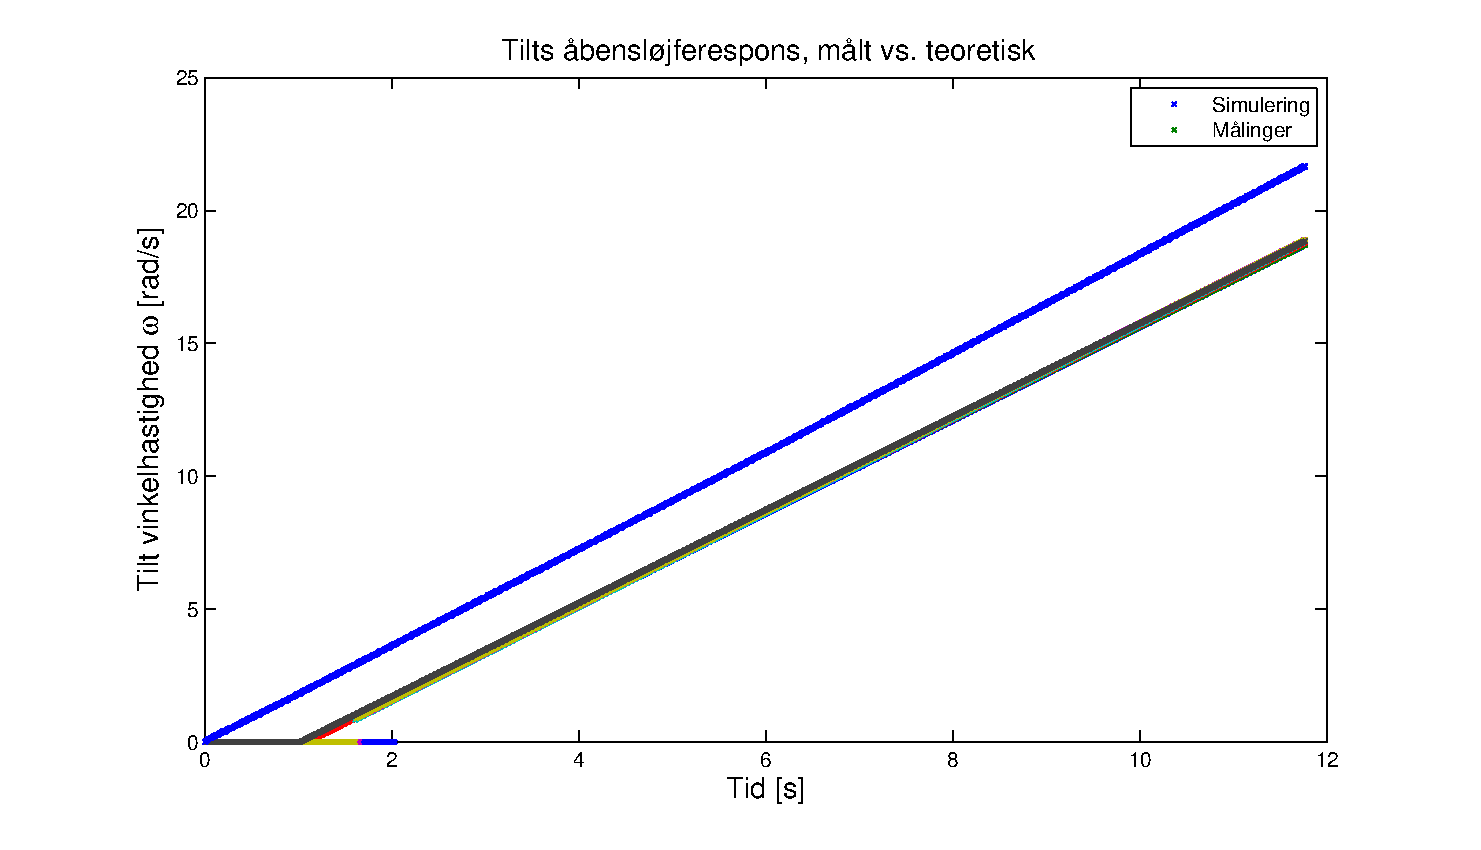
\includegraphics[width=1\textwidth]{./graphics/openloopVelocity1.eps}
	\caption[Tilt åbensløjferespons, målt vs. teoretisk]
		{Tilt åbensløjferespons, målt vs. teoretisk.
		Markeret med rødt er den målte respons for alle syv målinger,
		mens den teoretiske respons for de samme syv inputs er markeret med blåt.}
	\label{fig:openloopV1}
\end{figure}

Figur \ref{fig:openloopV1} viser den målte vinkelhastighed samt den teoretiske vinkelhastighed,
som forudsagt af overføringsfunktionen \(s\cdot{}G_{tilt}\).
Det ses på figur \ref{fig:openloopV1}, at den største afvigelse er en tidsforsinkelse.
Dette skyldes, at visse PWM-duty cycles ikke kan bevæge systemet.
Dødzonen af PWM-duty cycles, der ikke kan accelerere Tilt-systemet er målt til at befinde sig inden for
ca. \(\pm\) 12 \%, og for Pan-systemet til ca. \(\pm\) 10 \%.
Udover forsinkelsen fra dødzonen kan man på figur \ref{fig:openloopV1} aflæse
at den målte vinkelacceleration (hældningen af grafen) er marginalt mindre end den teoretiske.
Det antages, at denne opførsel hovedsageligt skyldes Coulomb-friktion.

Hvis man ønsker en mere nøjagtig matematisk model af Pan \& Tilt-systemet
er det altså en mulighed at indsætte dødzonen og evt. den ekstra dæmpning i modellen.
Det vælges dog at benytte åbensløjfeoverføringsfunktionerne \(G_{pan}\) og \(G_{tilt}\)
som udgangspunkt for analysen der hører til regulatordesignet,
og udvide modellen hvis regulatoren ikke lever op til kravene.

\subsection{Koordinattransformation}
\label{sec:koordinattransformation}
De kartesiske koordinater \(P_c=\left[x, y, z\right]\) skal transformeres til sfæriske koordinater \(P_s=\left[\rho \text{ ; } \phi \text{ ; } \theta\right]\), hvor \(\phi\) og \(\theta\) bruges som vinkelbestemmelserne for hhv. tilt og pan og \(\rho\) er afstanden fra PTS til duen som funktion af tiden.
Til trackingen er kun \(\phi\) og \(\theta\) nødvendige.
Positionbestemmelsen som funktion af tiden for det kartesiske koordinatsæt er udredt i afsnit \ref{subsubsec:para}.
Idet vinklerne skal bestemmes i forhold til PTS's rotationscenter og ikke koordinatsystemets origo, skal PTS's rotationscenter trækkes fra; \(PTS=[\text{19,2 ; 0 ; 0,45}]\). 

\subsubsection{Kartesiske koordinater}
Koordinattransformationen tager udgangspunkt i den kartesiske stedvektor \(Pos\left(t\right) \), ligning \ref{eq:pf:vektorparabel3d} samt PTS's offset, ligning \ref{eq:pf:stedvektorparabel}.
\begin{align}
\begin{split}
{ P }_{ c }=Pos\left( t \right) -PTS = \left( \begin{matrix} - 9,34\cdot t-13,7 \\32,851\cdot t-19,3
\\-{ 4,91\cdot t }^{ 2 }+5,473\cdot t+2,6\end{matrix} \right) [\text{m}]
\label{eq:pf:stedvektorparabel}
\end{split}
\end{align}
%Før koordinattransformationen fra kartesiske til sfæriske koordinater vises et grafisk overblik af \(\phi\) og \(\theta\) %samt \(\rho\), figur \ref{fig:thetaphi_degree}. 
Sammenhængen mellem de kartesiske og de sfæriske koordinater kan ses på fig \ref{fig:thetaphi_degree}. 
Grundet PTS's offset er origo for det sfæriske koordinatsystem PTS's rotationscenter (skæringspunktet mellem de to rotationsakser).

\begin{figure}[!th]
\centering
\begin{tikzpicture}[scale=4]
\include*{./graphics/3d_in_xyz_plane}
\end{tikzpicture}
\caption[Sfærisk koordinatsystem til koordinattransformation]{Viser duens placering i det sfæriske rum som funktion af  \(\phi\), \(\theta\) og \(\rho\).}
\label{fig:thetaphi_degree}
\end{figure}

\subsubsection{Sfæriske koordinater}
Som det fremgår af problemformuleringen modtager PTS lerduens
position som kartetiske koordinationer med en frekvens på 120 [Hz].
Dette bevirker at transformationen fra kartesiske koordinater til
sfæriske koordinater gøres ud fra nedenstående ligning \ref{eq:sv_koordi}.
\begin{align}
\begin{split}
{ P }_{ s } =\left( \begin{matrix} \rho  \\ \phi  \\ \theta  \end{matrix} \right) =\left( \begin{matrix} \sqrt { { { P }_{ c_{ x } } }^{ 2 }+{ { P }_{ c_{ y } } }^{ 2 }+{ { P }_{ c_{ z } } }^{ 2 } }  \\ { tan }^{ -1 }\left( \frac { \sqrt { { { P }_{ c_{ x } } }^{ 2 }+{ { P }_{ c_{ y } } }^{ 2 } }  }{ { P }_{ c_{ z } } }  \right)  \\ { tan }^{ -1 }\left( \frac { { P }_{ c_{ y } } }{ { P }_{ c_{ x } } }  \right)  \end{matrix} \right) %\\
 %&=\left( \begin{matrix} \sqrt { { \left( -9,34\cdot t-13,7 \right)  }^{ 2 }+{ \left( 32,851\cdot t-19,3 \right)  }^{ 2 }+{ \left( -{ 4,91\cdot t }^{ 2 }+5,473\cdot t+2,6 \right)  }^{ 2 } }  \\ { tan }^{ -1 }\left( \frac { \sqrt { { \left( -9,34\cdot t-13,7 \right)  }^{ 2 }+{ \left( 32,851\cdot t-19,3 \right)  }^{ 2 } }  }{  -{ 4,91\cdot t }^{ 2 }+5,473\cdot t+2,6 }  \right)  \\ { tan }^{ -1 }\left( \frac { 32,851\cdot t-19,3 }{ -9,34\cdot t-13,7 }  \right)  \end{matrix} \right) 
\label{eq:sv_koordi}
\end{split}
\end{align}
hvor \(\rho\) er afstanden i meter, \(\phi\) og \(\theta\) er angivet i grader, \citep[Kap. 10.6]{adam}.

\section{Regulator}
\label{sec:kontrollerdeign}
Det er valgt at designe regulatoren efter processen illustreret i figur \ref{fig:designproces}.
\begin{figure}[!th]
\centering
\include*{./graphics/designproces}
\caption[Designprocessen]{Designprocessen, \citep{reg_modern_control_systems}.}
\label{fig:designproces}
\end{figure}
Formålet med reguleringen er som beskrevet i afsnit \ref{sec:problemformulering},
at kontrollere pan- og tilt-rammernes position, så de tracker en lerdue.
Dette gøres ved styring af deres hastighed, ved at justere spændingsfaldene over de
to DC-motorer. Spændingsfaldene styres af PWM-generatorer, og regulatoren
kan derfor styre motorernes hastighed ved at vælge PWM-signalernes duty cycles.

I afsnit \ref{sec:kravspecifikation} opstilles kravene til systemets respons.
Disse er for en 1-radian reference opsummeret nedenfor.
\begin{itemize}
\item \(t_{s} \leq 0,557 \mathrm{\left[s\right]}\) (Settling Time)
\item \(SSE \leq 1,78 \%\) (Steady State Tracking Error)
\item \(P.O. \leq 134 \%\) (Overshoot i procent)
\end{itemize}

Det er fastlagt i projektoplægget, at regulatoren skal implementeres på mikrocontrolleren.
Da systemet som input modtager kartesiske koordinater,
skal der også på mikrocontrolleren foregå en koordinattransformation
til den logiske vinkelrepræsentation med sfæriske koordinater.
Systemets konfiguration består altså af en koordinattransformation,
en regulering, en aktuering og en positionsmåling, som illustreret
i figur \ref{fig:digitalkontroller1}.
Bemærk at denne konfiguration er for ét SISO-undersystem (enten pan eller tilt),
og at mikrocontrolleren skal regulere begge SISO-undersystemer.
\begin{figure}[!th]
\centering
\begin{tikzpicture}[auto, node distance=2.6cm,>=latex']
\include*{./graphics/digitalkontroller1}
\end{tikzpicture}
\caption[Systemkonfiguration]{Systemkonfiguration}
\label{fig:digitalkontroller1}
\end{figure}
Som beskrevet i afsnit \ref{sec:problemformulering},
så er input-samplingen fastlagt til at foregå med en frekvens på 60 [Hz].
Men som illustreret på figur \ref{fig:digitalkontroller1}, så skal reguleringssløjfen
"køres" (sample) med en frekvens \(f_s=\frac{1}{T_s}\), der ikke nødvendigvis er 60 [Hz].
Dvs. A/D- og D/A-konverteringerne skal foregå med frekvensen \(f_s\).

Der er overordnet to strategier til valg af samplingfrekvensen \(f_s\) hvormed
reguleringssløjfen skal køre.
Hvis man designer en kontinuert regulator til det kontinuerte domæne, så
skal diskretiseringen af controlleren være så tæt på den kontinuerte regulator som muligt.
Det vil sige, samplingfrekvensen skal vælges så høj som mulig.
Hvis man derimod designer en diskret regulator til det diskrete domæne,
så er diskretiseringen allerede foretaget inden designet af regulatoren.
Dvs. man finder en diskretiseret model af det fysiske system inden designet af regulatoren.
Kravet til diskretiseringen af åbensløjfeoverføringsfunktionerne er, at den diskrete repræsentation
skal være tilfredsstillende tæt på de kontinuerte overføringsfunktioner.
Hvis den diskrete overføringsfunktion eksempelvis afviger 20 \% fra den kontinuerte, ville man
sandsynligvis overveje at benytte en højere samplingfrekvens til diskretiseringen.
Sammenligningen af den diskrete overførselsfunktion og den kontinuerte overføringsfunktion
kan være både i tidsdomænet (fx steprespons) og i frekvensdomænet (frekvensrespons, fx. Bode-plots).




\begin{figure}[!th]
\centering
\begin{tikzpicture}[auto, node distance=2.6cm,>=latex']
\include*{./graphics/digitalkontroller2}
\end{tikzpicture}
\caption[tekst i indholdsfortegnelsen]{figurtekst}
\label{fig:}
\end{figure}

\begin{figure}[!th]
\centering
\begin{tikzpicture}[auto, node distance=2.6cm,>=latex']
\include*{./graphics/digitalkontroller3}
\end{tikzpicture}
\caption[tekst i indholdsfortegnelsen]{figurtekst}
\label{fig:}
\end{figure}
\section{Koordinattransformation}
\label{sec:koordinattransformation}


\citep[Kap. 10.6, s. 598]{adam}
